%capitulo08
\label{cap:schedule}
\noindent 

This section presents the schedule of activities for the development of this doctoral research project, starting in April of 2016 and ending in March 2020, totalling a period of 48 months. The dependence between the steps can lead, at some point, to changes in the schedule, and its restructuring is necessary. The activities of the nearest steps have a more detail level than those of the later steps, which are in a higher level of abstraction, because, as discussed in Section~\ref{cap:methodology}, with each step start, there is a planning in which discussed and listed the next activities and artefacts produced.
The focus of research from the present moment will be on the choice of approach to the research problems described in  Section~\ref{cap:researchproblems}.
Table~\ref{tab:schedule1} presents the planning of the academic training activities and the planning of the research activities.

\begin{table*}[htbp]
	\centering
	\caption{Schedule of activities.}
    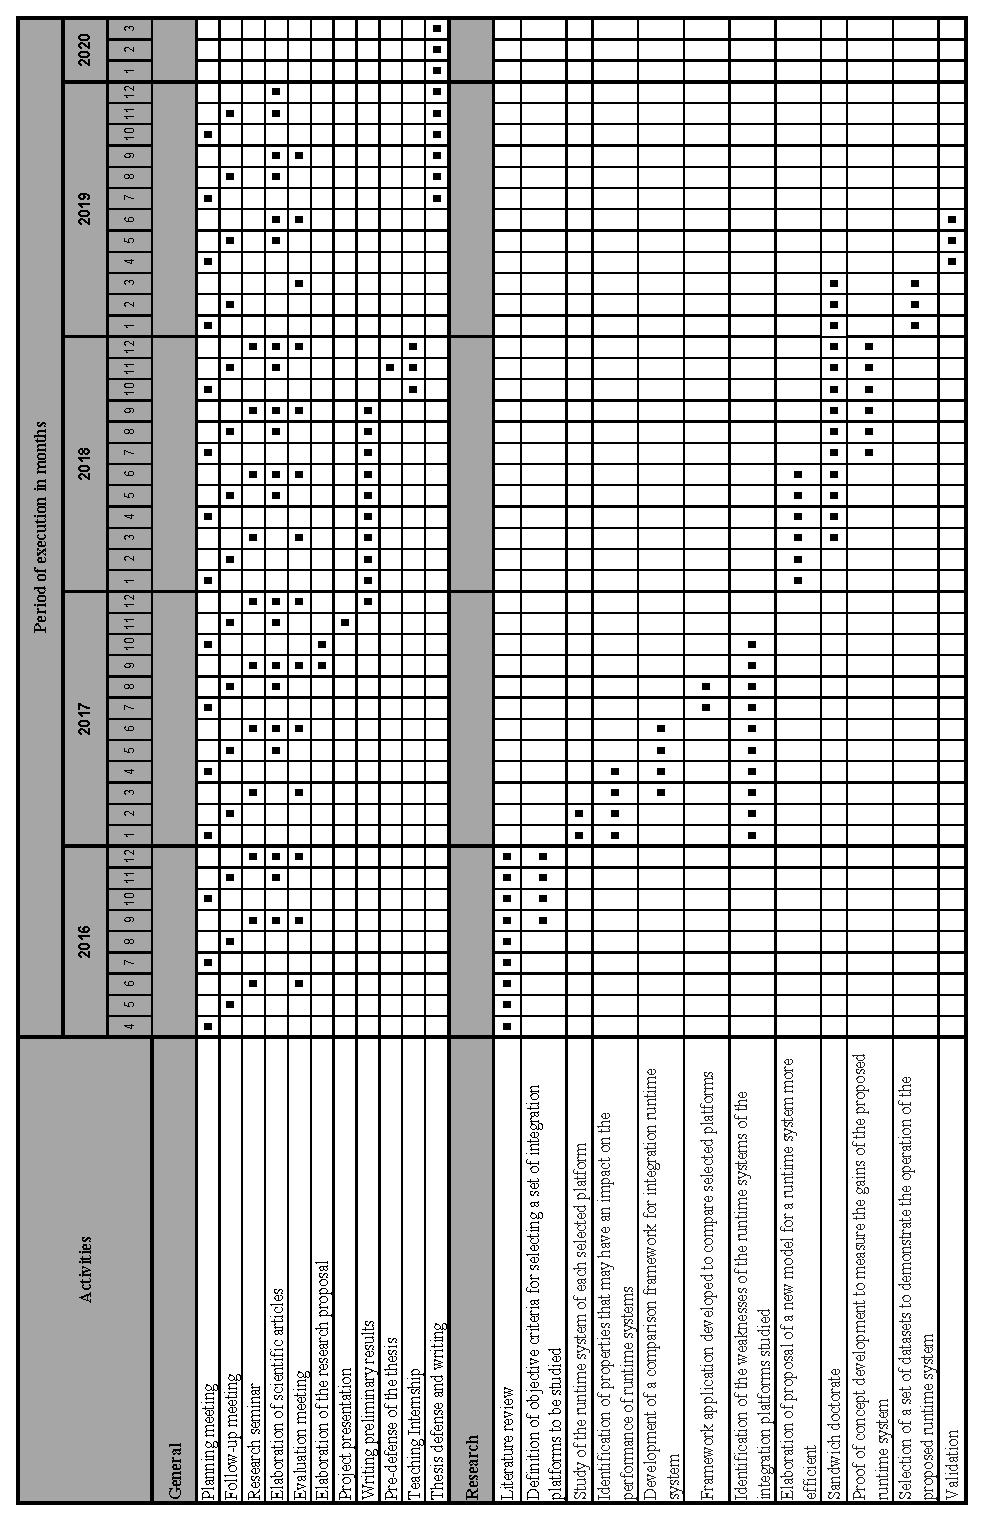
\includegraphics[scale=0.95]{./figs/schedule.eps}
	%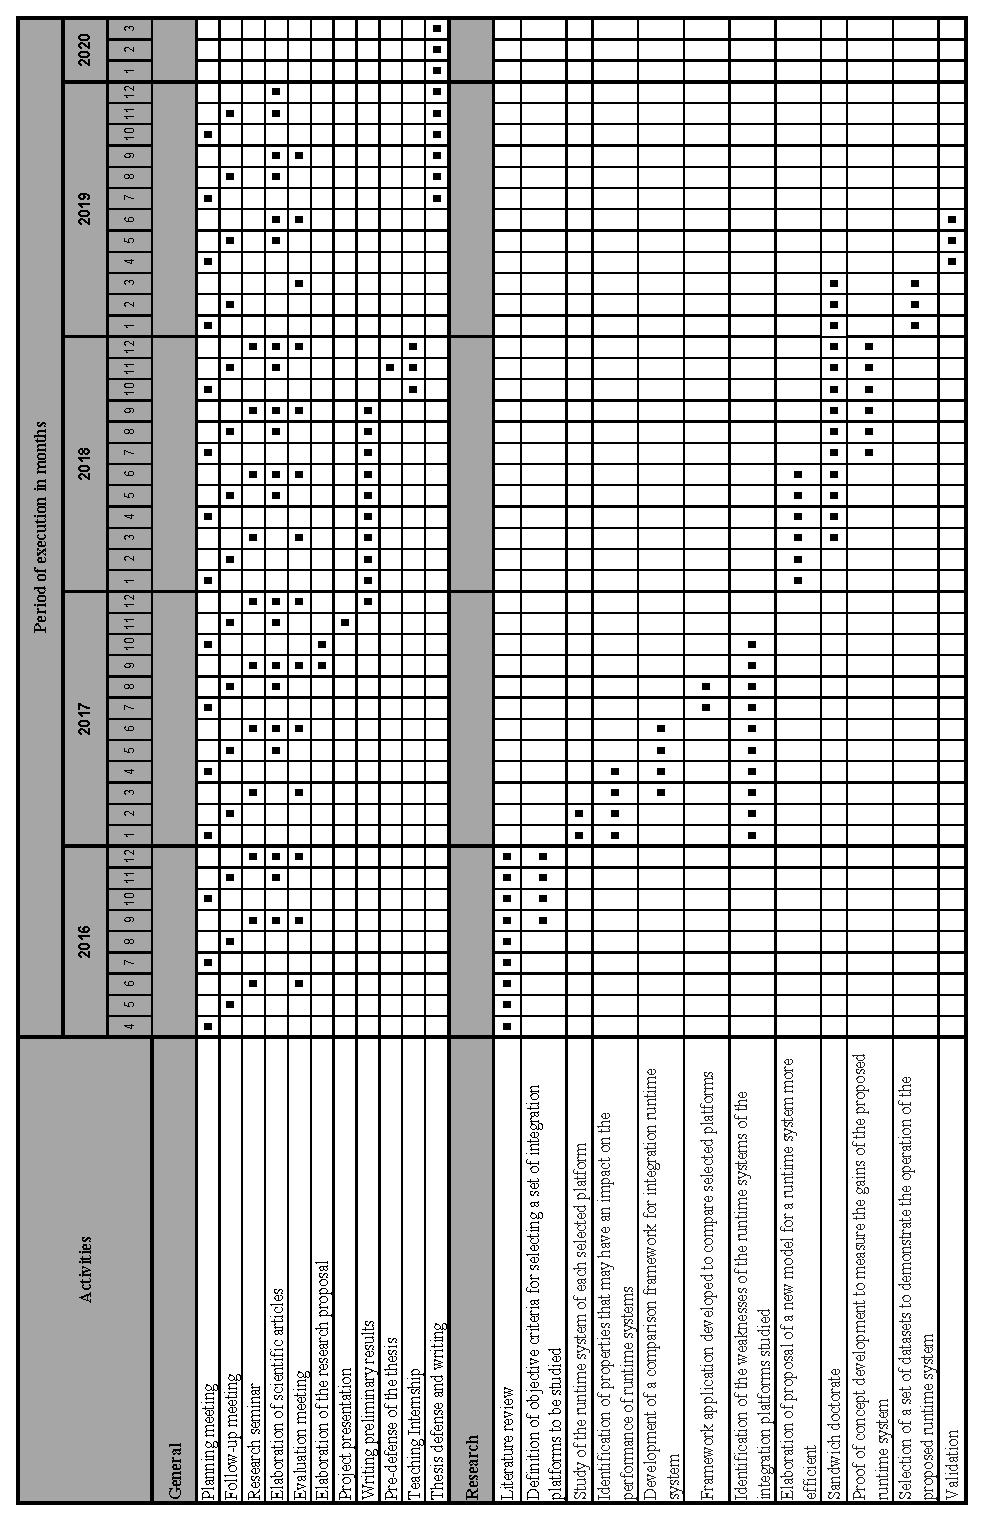
\includegraphics[width=\linewidth]{./figs/schedule.eps}
	\label{tab:schedule1}
\end{table*}

%current stage
In the first year of the research, we studied o research context, including EAI, runtime system, cloud computing and big data. After, we did a deep literature review in order to expand knowledge in the research fields: mathematical modelling, optimization techniques, statistics models and multithread programming. These knowledge form the foundation of our research.
Parallel, we determined criteria for selecting a set of integration platforms to be studied.

From the second year of research, we studied the runtime system of the selected platform e found properties that may have an impact on the performance of runtime systems. With that, we can development of a comparison framework for integration runtime system and apply it in the comparison of platforms, and finally, identified weaknesses of the runtime systems. The result generated a partial technical report. During this period, we produced peripheral works, which can lead or contribute to the solutions to the research questions.

We are begging a step third of research that is an elaboration of a proposal of a new model for a runtime system more efficient.